\documentclass[border=4pt]{standalone}
\usepackage{pgfplots}
\pgfplotsset{compat=1.18}

\begin{document}
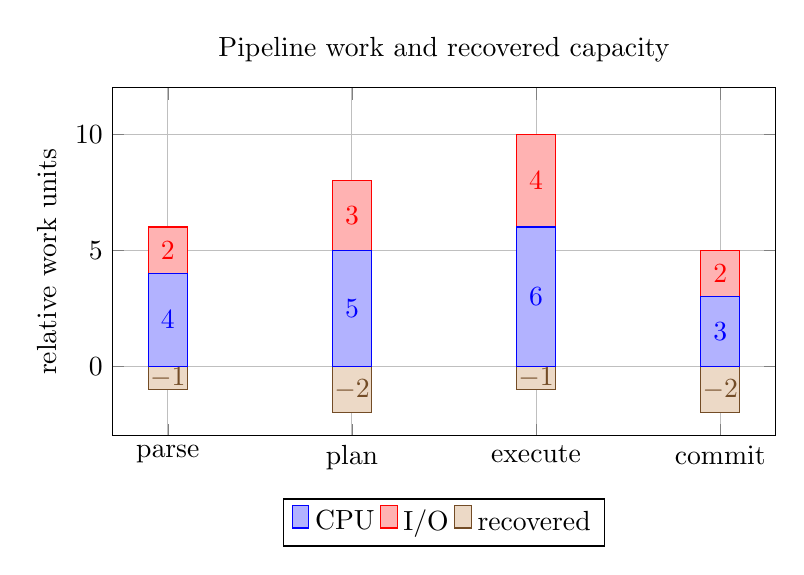
\begin{tikzpicture}
  \begin{axis}[
    ybar stacked,
    width=10cm,
    height=6cm,
    bar width=14pt,
    ymin=-3,
    ymax=12,
    xtick={1,2,3,4},
    xticklabels={parse,plan,execute,commit},
    ylabel={relative work units},
    title={Pipeline work and recovered capacity},
    grid=major,
    nodes near coords,
    legend style={at={(0.5,-0.18)},anchor=north,legend columns=-1}
  ]
    \addplot coordinates {(1,4) (2,5) (3,6) (4,3)};
    \addplot coordinates {(1,2) (2,3) (3,4) (4,2)};
    \addplot coordinates {(1,-1) (2,-2) (3,-1) (4,-2)};
    \legend{CPU,I/O,recovered}
  \end{axis}
\end{tikzpicture}
\end{document}
